% % Font size chart
% https://latex-tutorial.com/changing-font-size

% % Font size hierarcy
% tiny < scriptsize < footnotesize < small < normalsize < large < Large < LARGE < huge < Huge

% % Changing default element names
% https://tex.stackexchange.com/questions/82993/how-to-change-the-name-of-document-elements-like-figure-contents-bibliogr

\documentclass[a4paper, hidelinks, 12 pt, table]{article}
% Useful packages, sorted so packages of similar functionality are grouped together. Not all are essential to make the document work, however an effort was made to make this list as minimalistic as possible. Feel free to add your own!

% Essential for making this template work are graphicx, float, tabularx, tabu, tocbibind, titlesec, fancyhdr, xcolor and tikz. 

% Not essential, but you will have to debug the document a little bit when removing them are amsmath, amsthm, amssymb, amsfonts, caption, subcaption, appendix, enumitem, hyperref and cleveref.

% inputenc, lipsum, booktabs, geometry and microtype are not required, but nice to have.

\usepackage[utf8]{inputenc} % Allows the use of some special characters
\usepackage{amsmath, amsthm, amssymb, amsfonts} % Nicer mathematical typesetting
\usepackage{mathptmx} % For fonts
\usepackage{longtable} % For Long Tables spanning across pages
\usepackage{times} % For fonts
\usepackage{lipsum} % Creates dummy text lorem ipsum to showcase typsetting 
\usepackage[utf8]{inputenc}
\usepackage{hyphenat} % wordwrap with hyphens
\usepackage[T1]{fontenc}
\usepackage{parskip} % for paragraph spacing
\usepackage{graphicx} % Allows the use of \begin{figure} and \includegraphics
\usepackage{float} % Useful for specifying the location of a figure ([H] for ex.)
\usepackage{caption} % Adds additional customization for (figure) captions
\usepackage{subcaption} % Needed to create sub-figures
\usepackage{fontawesome5} % Needed for icons
\usepackage{tabularx, array} % Adds additional customization for tables
\usepackage{tabu} % Adds additional customization for tables
\usepackage{booktabs} % For generally nicer looking tables

\usepackage[nottoc,numbib]{tocbibind} % Automatically adds bibliography to ToC
% \usepackage[margin = 2.5cm]{geometry} % Allows for custom (wider) margins
\usepackage{microtype} % Slightly loosens margin restrictions for nicer spacing  
\usepackage{titlesec} % Used to create custom section and subsection titles
\usepackage{titletoc} % Used to create a custom ToC
\usepackage{appendix} % Any chapter after \appendix is given a letter as index
\usepackage{fancyhdr} % Adds customization for headers and footers
\usepackage[shortlabels]{enumitem} % Adds additional customization for itemize. 

\usepackage[hidelinks]{hyperref} % Allows links and makes references, and the ToC clickable
\hypersetup{
    colorlinks = false,
    linkcolor = black,
    % filecolor = black,
    urlcolor = black,
    % mailcolor = black
}

% \usepackage[
%     backend = bibtex, % biber,
%     style = ieee,
% ]{biblatex}
% \addbibresource{General/References.bib}

\usepackage[noabbrev, capitalise]{cleveref} % Easier referencing using \cref{<label>} instead of \ref{}
\usepackage{xcolor} % Predefines additional colors and allows user-defined colors
\usepackage{adjustbox} % Fitting figures and tables inside the page width
\usepackage{mathtools} % To use box inside an aligned environment
\usepackage{blindtext}
\usepackage{pgf, pgffor}

\usepackage{geometry, lipsum}

\geometry {
    top = 1.2 in,
    bottom = 1.4 in,
    left = 1.2 in,
    right = 1.2 in
}

% Allotting space for the header
\setlength{\headheight}{20pt}%

% Defines a command used by tikz to calculate some coordinates for the front-page
\makeatletter
\newcommand{\gettikzxy}[3]{%
  \tikz@scan@one@point\pgfutil@firstofone#1\relax
  \edef#2{\the\pgf@x}%
  \edef#3{\the\pgf@y}%
}
\makeatother

\usepackage{tikz} % Useful for drawing images, used for creating the frontpage
\usetikzlibrary{positioning} % Additional library for relative positioning 
\usetikzlibrary{calc} % Additional library for calculating within tikz
\usetikzlibrary{shapes.geometric, arrows}

% Defining Tickz Style
\tikzstyle{startstop} = [rectangle, rounded corners, minimum width=2cm, minimum height=1cm, text centered, text width = 8cm, draw=black, fill=white]

% \tikzstyle{io} = [trapezium, trapezium left angle=70, trapezium right angle=110, minimum width=3cm, minimum height=1cm, text centered, text width = 4.5cm, draw=black, fill=blue!30]

\tikzstyle{process} = [rectangle, minimum width=2cm, minimum height=1cm, text centered, text width = 8cm, draw=black, fill=white]

% \tikzstyle{decision} = [diamond, minimum width=3cm, minimum height=1cm, text centered, draw=black, fill=green!30]

\tikzstyle{arrow} = [ultra thick,->,>=stealth] % Loads in the preamble 
% Give your report a title
\newcommand\reporttitle{\textbf{Mini Project Report}}
\newcommand\group{\textbf{Group - B1}}

% Add an experiment number
% \newcommand\expno{\textbf{Experiment No. 1}}

% Insert course code, name, quartile number, and year (or any other subtitle)
\newcommand\reportsubtitle{
    \textbf{Machine Learning based short-term\\ forecasting of Orange and Cotton crop\\ prices in context of Indian market\\}
}

% Date and location (default: current date and YCCE, Nagpur)
\newcommand\placeanddate{
    \color{black}
    {
\includegraphics[width=0.1\paperwidth]{Figures/Logos/YCCE.png}}\\
    \vspace{10pt}
    % \today
    {October, 2023}\\
    \vspace{10pt}
    \textbf{
        Department of Computer Technology\\
        \vspace{10pt}
        Yeshwantrao Chavan College of Engineering\\
        Wanadongri, Nagpur, Maharashtra, India - 441110\\
    }    
    % \vspace{1.6 cm}
}

% Define theme-color (color of the logo). Can be changed to drastically change the look of the template

% % aqua
% \definecolor{theme-color}{RGB}{0, 128, 255}
% olive
% \definecolor{theme-color}{RGB}{0, 168, 89}
% % rose
% \definecolor{theme-color}{RGB}{248, 194, 217}
% % brass
% \definecolor{theme-color}{RGB}{153, 145, 62}
% % black
\definecolor{theme-color}{RGB}{0, 0, 0}

% Formats section, subsection and subsubsection titles
% % \titleformat{<command>}[<shape>]{<format>}{<label>}{<sep>}{<before-code>}[<after-code>]
\titleformat{\section}{\color{theme-color}\Large\raggedleft}{\thesection\enskip}{0 pt}{\fontfamily{cmr}\scshape\bfseries}{}{} % Formats section titles
\titleformat{\subsection}{\color{theme-color}\large\bfseries}{\thesubsection\enskip}{0 pt}{\fontfamily{cmr}\scshape\bfseries} % Formats subsection titles
\titleformat{\subsubsection}{\color{theme-color}\bfseries}{\thesubsubsection\enskip}{0 pt}{\fontfamily{cmr}\scshape\bfseries} % Formats subsubsection titles

% Settings for paragraph spacing 
\titlespacing*{\section}{0 pt}{0 pt}{4\baselineskip}
\titlespacing*{\subsection}{0 pt}{\baselineskip}{0.5\baselineskip}
\titlespacing*{\subsubsection}{0 pt}{\baselineskip}{0.5\baselineskip}
\setlist{nolistsep, leftmargin = 2 em}

% Table Settings
\newcolumntype{M}[1]{>{\sloppy\arraybackslash}m{#1}}
\newcolumntype{J}[1]{>{\justifying\sloppy\arraybackslash}X}

% Settings for figure size
\newcommand{\figsize}{0.24\textwidth}

% All of the following code can be removed to be left with (close to) default LaTeX behavior. 

% Sets up hyperlinks in the document to be colored
\hypersetup{
    colorlinks=true,
    linkcolor=theme-color,
    urlcolor=theme-color,
    citecolor = theme-color
}
\urlstyle{same} % Defines settings for link and reference formatting


% Change bullet style for level 1, 2 and 3 respectively for itemize
\renewcommand{\labelitemi}{\scriptsize\textcolor{theme-color}{$\blacksquare$}}% level 1
\renewcommand{\labelitemii}{\scriptsize\textcolor{theme-color}{$\square$}}% level 2
\renewcommand{\labelitemiii}{\textcolor{theme-color}{$\circ$}}% level 3

% Change bullet style for level 1, 2 and 3 respectively for enumerate
\renewcommand{\labelenumi}{\textbf{\textcolor{theme-color}{\arabic*.}}}% level 1
\renewcommand{\labelenumii}{\textbf{\textcolor{theme-color}{[\alph*]}}}% level 2
\renewcommand{\labelenumiii}{\textbf{\textcolor{theme-color}{\roman*.}}}% level 3

% Have reference labels be linked to section (section 3 will have fig. 3.1 etc.)
\counterwithin{equation}{section} % For equations
\counterwithin{figure}{section} % For figures
\counterwithin{table}{section} % For tables

% Creates a beautiful header/footer
% \pagestyle{fancy}
% \lhead{\group { | }\reporttitle}
% \rhead{
\includegraphics[height = 20pt]{Figures/Logos/YCCE Logo (BW).png}}
% \renewcommand{\footrulewidth}{0.4pt}
\cfoot{\thepage}


% Formats captions
\DeclareCaptionFont{theme-color}{\color{theme-color}}
\captionsetup{labelfont={theme-color,bf}}

 % Changes font to mlmodern
\usepackage{mlmodern}

% Removes indent when starting a new paragraph
\setlength\parindent{0pt}

% Limits the ToC to sections and subsections (no subsubsec.)
\setcounter{tocdepth}{2} % Loads in user defined settings
% \usepackage[none]{hyphenat}

% \setmainfont{Times New Roman}
% \setmainfont{Times New Roman}[
%     SmallCapsFont = {TeX Gyre Termes},
%     SmallCapsFeatures = {Letters = SmallCaps},
% ]

\renewcommand{\contentsname}{
    \begin{center}
        \huge{Contents}
    \end{center}
}

\begin{document}

    \sloppy
    
    % % Serif Family Computer Modern
    % \sffamily
    % \renewcommand{\rmdefault}{\sfdefault}
    
    % % Times New Roman
    % \fontfamily{ptm}\selectfont
    % \renewcommand{\rmdefault}{}
    
    % \newpage
    % \newgeometry {
    top = 1 in,
    bottom = 1 in,
    left = 0.6 in,
    right = 0.6 in
}

\begin{titlepage}

    \centering
    % \sffamily

% \includegraphics[width=.36\textwidth]{Figures/Logos/SIH 2023.png}

% \vspace{8 cm}

{\Large \reporttitle}\\

% {\large \expno}
\vspace{1 em}
on
\vspace{1 em}

{\LARGE \reportsubtitle}\\

\vspace{4 em}

\begin{table}[H]
    \centering
    % \sffamily
        Submitted by\\
    \large
        \vspace{1 em}
    \begin{tabu} to \linewidth {C C C C C}
        
        \textbf{Student Name} & \textbf{Enrollment No.} & \textbf{Semester} & \textbf{Section} & \textbf{Roll No.}\\
        Mr. Humanshu D G & 20010635 & VII & B & 147\\
        Mr. Susrut Patole & 20010522 & VII & B & 169\\
        Ms. Neha Thakur & 20010732 & VII & B & 110\\
        Ms. Geetika Mahant & 20010191 & VII & B & 102
    \end{tabu}
\end{table}

\vspace{4 em}

\begin{table}[H]
    \centering
    % \sffamily
        Under the guidance of\\
    \large
        \vspace{1 em}
    \begin{tabu} to \linewidth {C}
        \textbf{Prof. (Dr.) Nileshsingh V. Thakur}
    \end{tabu}
\end{table}

% \tikz[remember picture, overlay, opacity = 0.11]\node[anchor = south, inner sep = 0 pt] at (current page.south) {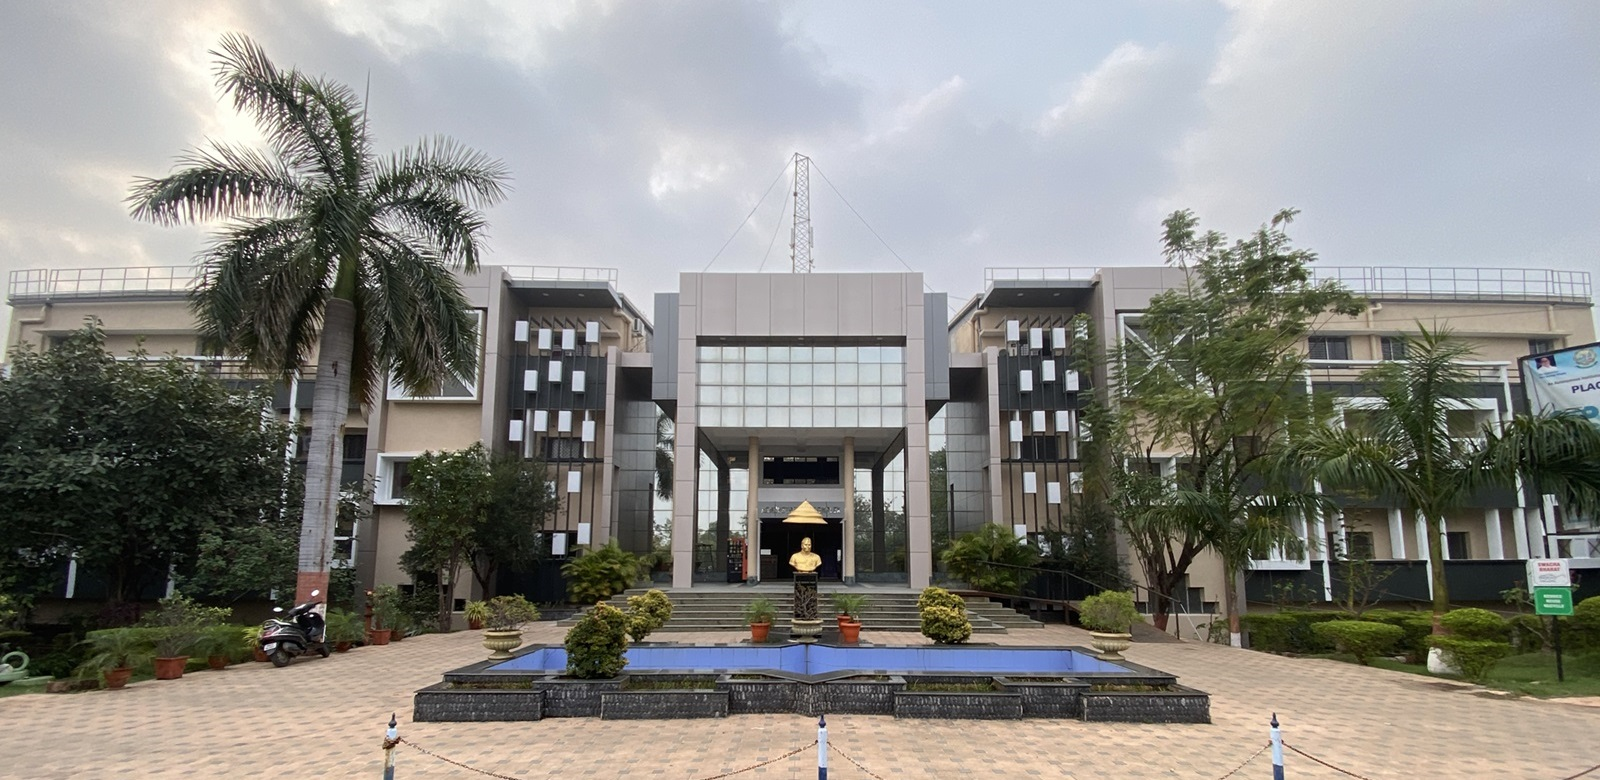
\includegraphics[width=\paperwidth]{Figures/Logos/YCCE Main Building tall.jpg}};

\mbox{}
    \vfill
    % \sffamily
    \large
    \textcolor{white}{\placeanddate}
\end{titlepage}
    % \newpage
    % \newgeometry {
    top = 1 in,
    bottom = 1 in,
    left = 1 in,
    right = 1 in
}
\thispagestyle{empty}
\pagenumbering{roman}

\begin{certificate}

    \begin{center}
        \parbox{\textwidth}{
            % \hspace{0.02\textwidth}
            \hspace{0.01\textwidth}
            \parbox{0.12\textwidth}{
                
\includegraphics
                    [width = 0.12\textwidth, clip]
                    {Figures/Logos/YCCE.png}
            }
            \hspace{0.01\textwidth}
            \parbox{0.9\textwidth}{ %\dimexpr\relax\linewidth
                % \hspace{2 mm}
                \setlength{\tabcolsep}{0 pt}
                \begin{tabularx}{0.896\textwidth}[t]{C}
                    \tiny{Nagar Yuwak Shikshan Sanstha’s}\\
                    \textbf{\Large{Yeshwantrao Chavan College of Engineering}}\\
                    \scriptsize{(An Autonomous Institution Affiliated to Rashtrasant Tukadoji Maharaj Nagpur University)}\\
                    \small{Hingna Road, Wanadongri, Nagpur - 441110}\\
                    \scriptsize{\textcolor{red}{NAAC Accredited with \textbf{A\texttt{++}} Grade}}\\
                    \scriptsize{{\faPhone*} 07104 - 295083, 295085 \hspace{1 em} {\faGlobe} \href{https://www.ycce.edu}{\textcolor{black}{www.ycce.edu}} \hspace{1 em} {\faEnvelope} {\href{mailto:principal@ycce.edu}{\textcolor{black}{principal@ycce.edu}}}, {\href{mailto:hod_ct@ycce.edu}{\textcolor{black}{hod\_ct@ycce.edu}}}}
                \end{tabularx}
            }
        }
        \hline
        \vspace{-2 pt}
        Department of Computer Technology
        \vspace{4 pt}
        \hline
        
        \vspace{2 em}
        
        \large{Session 2023 - 2024}
        
        \vspace{2 em}
        
        \LARGE{\textbf{Certificate}}\\
        
        \vspace{1 em}
    \end{center}
    
    \justifying\sloppy{
        This is to certify that the Mini Project Report titled \textbf{\textit{Machine Learning based short-term forecasting of Orange and Cotton crop prices in context of Indian market}} being submitted towards the partial fulfillment of the requirement of the Mini Project course in Semester - VII, Bachelor of Technology in Computer Technology is approved.
    }

    % \vspace{2 em}
    
    Submitted by:\\
    \begin{table}[H]
        % \sffamily
        \centering
            \vspace{-2 em}
        \begin{tabu} to \linewidth {C C C C}
            \textbf{Student Name} & \textbf{Enrollment No.} & \textbf{Section} & \textbf{Roll No.}\\
            Mr. Humanshu D G & 20010635 & B & 147\\
            Mr. Susrut Patole & 20010522 & B & 169\\
            Ms. Neha Thakur & 20010732 & B & 110\\
            Ms. Geetika Mahant & 20010191 & B & 102
        \end{tabu}
    \end{table}

    % \vspace{1 em}
    
    \begin{table}[H]
        % \centering
        % \sffamily
        \begin{tabu} to \linewidth {r l}
            \textbf{Date} & \rule{80pt}{0.1pt}\\
            \textbf{Place} & \rule{80pt}{0.1pt}
        \end{tabu}
    \end{table}
    % }
    \begin{table}[b]
            \centering
            % \sffamily
            \setlength{\tabcolsep}{6 pt}
            \begin{tabu} to \linewidth {C C C}
                {\hrulefill} & {\hrulefill} & {\hrulefill}\\
                {Prof. (Dr.) Nileshsingh V. Thakur} & {Mrs. Smita R. Kapse} & {Dr. Rakhi D. Wajgi}\\
                \textbf{Project Guide} & \textbf{Project Coordinator} & \textbf{Head of Department}
            \end{tabu}
        \end{table}
\end{certificate}
    % \newpage
    % \newgeometry {
    top = 2 in,
    bottom = 2 in,
    left = 2 in,
    right = 2 in
}
\thispagestyle{empty}

\begin{acknowledgement}
    
    \begin{center}
        \huge{Acknowledgement}
    \end{center}
    
    \vspace{2 em}
    \normalsize \justifying \sloppy
    
    We would like to thank our Project Guide for thorough guidance in the project. We are extremely grateful and indebted to them for their expert, sincere, valuable guidance and encouragement which was of immense help to us.\\

    \\
    
    We would like to express our sincere gratitude to the Head, Department of Computer Technology for their constant encouragement towards the successful completion of our work.\\

    \\
    
    We wish to express our sincere thanks to the Principal of our college for providing us with all the necessary facilities and the infrastructure without which we would not have been able to complete our project successfully.\\

    \\
    
    We would also like to thank our Project Coordinator for their continuous guidance owing to which the project could take shape.\\

    \\
    
    We would like to thank Technical Assistant for providing necessary technological support. Last, but not the least, we would like to thank all the faculty members and non-teaching staff members who helped us despite of their busy schedule.
    
\end{acknowledgement}
    % \newpage
    % \newgeometry {
    top = 2 in,
    bottom = 1 in,
    left = 1 in,
    right = 1 in
}
\renewcommand{\abstractname}{}
% \renewcommand{\absnamepos}{empty}

\begin{abstract}
    
    \addmargin
    
    \begin{center}
        \huge{Abstract}
        \vspace{2 em}
    \end{center}

    \it
        This project endeavours to construct a Machine Learning-based model tailored to the short-term forecasting of orange and cotton crop prices in the Indian market. Leveraging an extensive dataset provided by the Indian Government, the project initiates with a pivotal phase of Exploratory Data Analysis (EDA). This process serves to address the challenges posed by missing data and, importantly, to unveil latent patterns inherent in the dataset.
        
        A key aspect of the project is data preparation and partitioning. The dataset is meticulously split into training, testing, and validation sets to facilitate the subsequent model development and evaluation phases.
        
        The forecasting methodology encompasses a spectrum of regression-based algorithms, including Artificial Neural Networks (ANN), Auto Regressive Integrated Moving Average (ARIMA), Logistic Regression (LR), and Support Vector Regression (SVR). Additionally, an ARIMA model is incorporated for comparative assessment. These algorithms serve as the workhorses for our price prediction model.
        
        The analysis extends beyond mere algorithm selection. Regional and seasonal dynamics are incorporated into the model's framework. The dataset is categorized into urban and rural segments to account for regional variations. Notably, model performance and accuracy are evaluated at different geographical granularities, including the national, state, and city levels, to provide a comprehensive understanding of the price prediction capability.
        
\end{abstract}
    
    % Generates a ToC without page number
    {\hypersetup{linkcolor=black} % Keeps the ToC black even with non-black linkcolor
    \newpage
    \tableofcontents\thispagestyle{empty}}

    \newgeometry {
        top = 1 in,
        bottom = 1 in,
        left = 1 in,
        right = 1 in
    }
    
    % Creates the introduction, starting page numbering
    \pagenumbering{arabic}
    
    \newpage
    \section{Introduction}

\subsection{Motivation}
India being majorly agrarian economy, farmers' livelihoods are greatly impacted by the pricing of crops like cotton and oranges. India is one of the largest producers and exporters of cotton and oranges in the world. These crops' prices are frequently unstable and change depending on a number of variables, including the weather, supply and demand, and governmental policy. Farmers and traders find it challenging to plan the timing of their product sales and purchases in light of these changes. Accurate crop price forecasts can assist farmers, dealers, and policymakers in making educated decisions. This issue is made worse by the absence of an accurate forecasting model for crop prices. Machine learning algorithms can be used to estimate future prices by analyzing past price trends and other pertinent data.

\subsection{Background}
\subsubsection{Agricultural Significance in India}
The agricultural sector in India is the backbone of the economy, supporting the livelihoods of a substantial portion of the population. The pricing of key crops, such as oranges and cotton, not only impacts farmers directly but also influences the overall economic landscape. Understanding and predicting the fluctuations in crop prices is paramount for informed decision-making and sustainable agricultural practices.

\subsubsection{Dataset Overview}
The project leverages a comprehensive dataset provided by the Indian Government, offering a historical perspective on crop prices across diverse regions and seasons. This dataset serves as the bedrock for the development and validation of machine learning models for short-term forecasting.

\subsection{Exploratory Data Analysis (EDA)}
    \begin{enumerate}
        \item Data Cleaning and Imputation\\
            Prior to analysis, a meticulous EDA is conducted to address missing data and ensure the integrity of the dataset. Techniques such as imputation and data cleaning are employed to enhance the quality of the dataset, laying the groundwork for accurate and reliable forecasting models.
        \item Pattern Identification\\
            The EDA phase aims to uncover inherent patterns within the data. Through statistical analyses and visualization techniques, the project seeks to discern trends, cyclical patterns, and any anomalies that may be indicative of the underlying dynamics governing crop prices.
    \end{enumerate}

\subsection{Geographic Segmentation}
    \begin{enumerate}
        \item Urban and Rural Tiers
            Recognizing the diversity of the Indian agricultural landscape, the dataset is segmented into tiers representing urban and rural cities. This segmentation allows for a nuanced examination of how regional disparities influence pricing dynamics, providing valuable insights for targeted interventions.
        \item State-Level Analysis
            The project delves into state-level dynamics, acknowledging the varied agricultural practices and market conditions across different states in India. This analysis contributes to a more localized understanding of the factors shaping crop prices.
        \item City-Specific Insights
            Further granularity is achieved by focusing on specific cities, allowing the project to unravel localized trends and intricacies. This micro-level analysis facilitates a fine-tuned evaluation of model accuracy and aids in tailoring strategies to address city-specific challenges.
    \end{enumerate}

\subsection{Model Development and Selection}
    \begin{enumerate}
        \item Regression-Based Algorithms\\
            Four candidate algorithms—Artificial Neural Network (ANN), AutoRegressive Integrated Moving Average (ARIMA), Logistic Regression (LR), and Support Vector Regression (SVR)—are chosen for their capacity to handle regression tasks. The inclusion of ARIMA serves as a benchmark, offering a basis for comparison against machine learning approaches.
        \item Training-Testing-Validation Sets\\
            The dataset is strategically partitioned into training, testing, and validation sets to enable rigorous evaluation of model performance. This ensures that the selected algorithms are not only accurate in their predictions but also generalize well to unseen data.        
    \end{enumerate}

\subsection{Comparative Analysis}
    \begin{enumerate}
        \item National Overview\\
            The project begins with a broad national analysis, providing a holistic understanding of crop price forecasting across the entire country. This sets the stage for subsequent, more detailed examinations at lower geographic levels.
        \item State-Level Performance\\
            The effectiveness of the forecasting models is assessed at the state level, allowing for the identification of regional variations and the validation of model robustness in diverse agricultural contexts.
        \item City-Specific Accuracy\\
            The project concludes with an exploration of city-specific insights, shedding light on how well the models perform in distinct urban and rural environments. This localized evaluation is crucial for tailoring strategies to address specific market conditions.            
    \end{enumerate}
    In summary, this project is a comprehensive exploration of machine learning-based short-term forecasting for orange and cotton crop prices in the Indian market. By incorporating geographic segmentation and seasonal considerations, the aim is not only to provide accurate predictions but also to offer actionable insights for stakeholders at different levels of the agricultural supply chain. Through this multifaceted approach, the project contributes to the ongoing efforts to enhance the resilience and sustainability of India's agricultural sector.
    
    \newpage
    \section{Aim and Objectives}

\subsection{Aim}
    To devise a Machine Learning based short-term forecasting mechanism of orange and cotton crop prices in context of Indian market.

\subsection{Objectives}
    The objective of this project is to create a machine learning-driven model for predicting the prices of orange and cotton crops within the Indian market.
    % The model should be able:
    \begin{enumerate}
        \item
            Perform exploratory data analysis to address missing data in the dataset.
        \item
            Identify patterns within the data, if any, that can inform the price prediction model.
        \item
            Devise a method to determine the appropriate number of data records for training the model.
        \item
            Explore various training and learning algorithms to identify the most suitable ones for the task.
        \item
            Test and validate the model to ensure its accuracy and reliability.
        \item
            Tuning the hyperparameters of the best performing model.
        \item
            Build a machine learning-based model for predicting the prices of orange and cotton crops in the Indian market.
    \end{enumerate}
    
    \newpage
    \section{Literature Review}
    \subsection{General Work}
        Casper Solheim Bojer. (2022) “Understanding machine learning-based forecasting methods: A decomposition framework and research opportunities”\cite{bojer}. The research paper titled "Understanding machine learning-based forecasting methods: A decomposition framework and research opportunities" by C.S. Bojer offers insights into the growing interest in machine learning-based forecasting methods. It highlights their successful applications in forecasting competitions like the M4, M5, and Kaggle, challenging traditional statistical methods. The paper underscores the need for a systematic understanding of these methods due to their complexity, with diverse components including preprocessing, feature engineering, and ensembling. It introduces a framework for regression-based machine learning forecasting, aiming to standardize terminology and abstraction for researchers. The framework is applied to map and compare winning solutions from the M5 Uncertainty competition, emphasizing the complexity of strategies employed. Additionally, the paper identifies research areas such as cross-learning, feature engineering, and cross-validation, signaling potential advancements in the field of machine learning-based forecasting.
        
        Gianluca Bontempi , Souhaib Ben Taieb, and Yann-A¨el Le Borgne (2013) “Machine Learning Strategies for Time Series Forecasting”. [2] The research paper titled "Machine Learning Strategies for Time Series Forecasting" authored by Gianluca Bontempi, Souhaib Ben Taieb, and Yann-Aël Le Borgne provides a comprehensive overview of the role of machine learning techniques in the field of time series forecasting. The paper addresses the growing demand for accurate forecasting across various domains and the transition from traditional linear statistical methods, such as ARIMA models, to machine learning models. It highlights the importance of formalizing one-step forecasting problems as supervised learning tasks and discusses the use of local learning techniques for handling temporal data. The paper explores various strategies for multi-step forecasting, including the Recursive, Direct, and Multiple Output (MIMO) strategies, each with its advantages and limitations. Additionally, the paper introduces the concept of the DIRMO strategy, which combines elements of both Direct and MIMO strategies, providing a flexible approach to multi-step forecasting. The authors also delve into the use of local learning techniques for improving long-term predictions within these strategies.
        
        Yitong Li, Kai Wu, Jing Liu (2023) “Self-paced ARIMA for robust time series prediction”.[3] The  ARIMA (autoregressive integrated moving average ) model is a widely respected and traditional linear model for time series prediction, known for its effectiveness in various domains. However, its vulnerability to noisy data, leading to instability and reduced performance, has not received sufficient attention. In this study, we introduce the spARIMA framework to enhance the reliability of time series prediction. We implement a sequential training approach in batches, taking into account noise levels and their impact on accurate modeling, with the goal of minimizing noise-related disruptions during training. To leverage the advantages of self-paced learning (SPL), spARIMA integrates a differential prediction model into the ARIMA framework.
        
        Ahmed Tealab, Hesham Hefny, Amr Badr (2017) “Forecasting of nonlinear time series using ANN”. [4] Since basic linear time series models often fall short in fully explaining certain aspects of economic and financial data, it becomes crucial to categorize time series based on their linearity characteristics when conducting forecasts. This approach ensures that linear time series continue to be the focal point of both academic and practical research. Predicting nonlinear time series, especially those containing inherent moving average components, using computational intelligence methods like neural networks can be challenging, given that real-world time series often exhibit dynamic behavior, autoregressive elements, and inherited moving average terms. Research focusing on the prediction of nonlinear time series with moving average components is relatively rare. In this study, we demonstrate that conventional neural networks struggle to effectively capture the behavior of nonlinear time series with moving average terms, resulting in subpar forecasting performance.
        
        Hanyu Yang a, Xutao Li a, Wenhao Qiang a, Yuhan Zhao a, Wei Zhang b, Chang Tang c (2021) “A network traffic forecasting method based on SA optimized ARIMA–BP neural network”.[5]It explores the domain of network traffic forecasting, emphasizing the challenges faced by traditional linear and non-linear models. The proposed method integrates Simulated Annealing (SA)-optimized AutoRegressive Integrated Moving Average (ARIMA) with Back Propagation Neural Network (BPNN) to enhance prediction accuracy. The research highlights the contribution of the approach in extracting both linear and non-linear features from network traffic data, addressing limitations in existing models. Notable advances include improved network congestion control mechanisms and enhanced accuracy in fields relying on precise network traffic predictions. Real-world datasets validate the superiority of the proposed method, showcasing its effectiveness against single and hybrid prediction models. The study also conducts sensitivity analysis, demonstrating the method's stability across varying temporal spans. Future directions involve considering user behavior impact, exploring additional factors, and applying the method in Software-Defined Networking (SDN) systems for automated adjustments based on predicted trends. In conclusion, the proposed SA-optimized ARIMA–BPNN method proves promising for various applications, offering superior accuracy in network traffic forecasting and addressing non-linear complexities.
        
        Jennifer L. Castle , Michael P. Clements, David F. Hendry (2014).“Robust approaches to forecasting ”.[6] The paper investigates robust approaches to forecasting, particularly focusing on a new class of robust devices in contrast to equilibrium-correction models. The authors explore the forecasting properties of these robust methods in the face of empirical challenges such as measurement errors, impulses, omitted variables, unanticipated location shifts, and incorrectly included variables. The study applies these robust approaches to forecast US GDP using autoregressive models and models with factors extracted from a large dataset of macroeconomic variables. The empirical analysis spans both the Great Recession and an earlier, more stable period, providing insights into the performance of robust forecasting devices under different economic conditions. The authors compare the proposed robust devices with traditional models like autoregression and factor models, evaluating their effectiveness in mitigating forecast failures caused by shifts in the economic environment. The results suggest that the robust devices, especially those with smoothing techniques, show promise in improving forecast accuracy, particularly in the face of significant economic shifts. The empirical findings contribute to the understanding of robust forecasting methods, emphasizing their potential advantages in handling real-world forecasting challenges.
        
        G. Peter Zhang (2002) “Time series forecasting using a hybrid ARIMA and neural network model”. [7] The research paper explores time series forecasting by proposing a hybrid methodology that combines the Autoregressive Integrated Moving Average (ARIMA) model with Artificial Neural Networks (ANNs). ARIMA has been a popular linear model in time series forecasting, while recent studies suggest that ANNs offer a promising alternative with flexible nonlinear modeling capabilities. The hybrid approach aims to leverage the strengths of both models to enhance forecasting accuracy. The motivation behind this combination arises from the challenges in determining whether a time series is linear or nonlinear, the presence of both linear and nonlinear patterns in real-world data, and the recognition that no single method is universally superior. The paper argues that the hybrid model addresses these issues and presents experimental results using real datasets to support its effectiveness. The literature review highlights the importance of model combination for improved forecasting accuracy, drawing on the well-known M-competition and emphasizing the benefits of combining dissimilar models to reduce generalization variance and model uncertainty. The authors position their work within the context of ongoing efforts to enhance time series forecasting methodologies.

    \subsection{Research Paper Study}
        The following table summarizes our research paper review in tabular form.
        % \scriptsize
        \setlength\tabcolsep{0.006\textwidth}
        \begin{longtable}[H]{@{}
        >{\centering\arraybackslash} M{0.06\textwidth}
        >{\justifying\arraybackslash} M{0.12\textwidth}
        >{\justifying\arraybackslash} M{0.2\textwidth}
        >{\justifying\arraybackslash} M{0.18\textwidth}
        >{\justifying\arraybackslash} M{0.12\textwidth}
        >{\justifying\arraybackslash} M{0.12\textwidth}
        >{\justifying\arraybackslash} M{0.14\textwidth}
        @{}}
            \toprule
                % \setlength\tabcolsep{0.0\textwidth}
                \multicolumn{1}{>{\centering\arraybackslash} M{0.06\textwidth}}{\textbf{Ref. No.}} & 
                \multicolumn{1}{>{\centering\arraybackslash} M{0.12\textwidth}}{\textbf{Work carried out}} & 
                \multicolumn{1}{>{\centering\arraybackslash} M{0.2\textwidth}}{\textbf{Methodology}} & 
                \multicolumn{1}{>{\centering\arraybackslash} M{0.18\textwidth}}{\textbf{Evaluation Metrics}} & 
                \multicolumn{1}{>{\centering\arraybackslash} M{0.12\textwidth}}{\textbf{Dataset}} & 
                \multicolumn{1}{>{\centering\arraybackslash} M{0.12\textwidth}}{\textbf{Claims}} & 
                \multicolumn{1}{>{\centering\arraybackslash} M{0.14\textwidth}@{}}{\textbf{Findings}}\\
            \toprule
            \endhead
                % % \begin{headers}
                %     \toprule
                %     \thead{Ref.\\No.} &
                %     \thead{Work carried out} &
                %     \thead{Methodology} &
                %     \thead{Evaluation Metrics} &
                %     \thead{Dataset} &
                %     \thead{Claims} &
                %     \thead{Findings}
                %     % {\textbf{Ref. No.}} & {\centering{\textbf{Work carried out}}} & {\centering{\textbf{Methodology}}} & 
                %     % \multicolumn{2}{c}{\textbf{Evaluation Metrics}}
                %     % % \centering{\textbf{Evaluation Metrics}}
                %     % & \centering{\textbf{Dataset}} & \centering{\textbf{Claims}} & \centering{\textbf{Findings}}
                % % \end{headers}
                % \endhead
                
                \cite{sami} &
                Mapping and comparing ML methods &
                Framework development, method mapping, performance assessment. &
                Mapping, comparison, ablation testing for evaluation. &
                Kaggle &
                Common language, improved forecasting methods. &
                Complexity understanding, needs further exploration.\\
                
                \bottomrule
            \caption{Literature Review - summary of research papers studied}
        \end{longtable}

    \newpage
    \subsection{Patent Study}
        The following table summarizes our patent review in tabular form.
        
        \setlength\tabcolsep{0.006\textwidth}
        \begin{longtable}[H]{@{}
        >{\centering\arraybackslash}M{0.22\textwidth}
        >{\justifying\sloppy\arraybackslash} M{0.18\textwidth}
        >{\justifying\sloppy\arraybackslash} M{0.586\textwidth}
        @{}}
                    \toprule
                    \multicolumn{1}{@{}>{\centering\arraybackslash}M{0.22\textwidth}}{\textbf{Application Number}} & 
                    \multicolumn{1}{>{\centering\sloppy\arraybackslash} M{0.18\textwidth}}{\textbf{Title}} & 
                    \multicolumn{1}{>{\centering\sloppy\arraybackslash} M{0.557\textwidth}@{}}{\textbf{Abstract}}\\
                    \toprule
                \endhead
                
                CN103577581B & Agricultural product price trend forecasting method & The technique of agricultural product price trend forecasting described in the invention includes the following steps. Step 1: computer-acquired article relevant to agricultural commodity price and with a forecasting standpoint; Step 2: Duplicate elimination is completed on the collected articles; Extract and save the article's important element in step three.Step 4: The location of the agricultural product-related area mentioned in the article is found; Step 5: Quantify and preserve agricultural products according to the given predictability viewpoint after analyzing expert opinions using text mining technology; Step 6: Utilizing the model established so that agricultural product price is carried out-trend prediction, the trend prediction viewpoint delivering time, agricultural product affiliated area, agricultural product sort, and quantization according to article is carried out using microcomputer modeling.\\
    
                \midrule
                
                CN105205099B & A kind of agricultural product price analysis method & The steps included in the technique of agricultural product price analysis that the present invention relates to are as follows: Information about the types of agricultural products is gathered using one assembled classifier of pre-trained search engines; The default commodities trading website is crawled to obtain the geographic location information of the supplier for each category of agricultural commodity as well as the pricing data .It is divided based on the  area where agricultural goods are cultivated, with each agricultural product kind carrying out agricultural production and obtaining information on the area where agricultural goods are cultivated for each kind.\\
    
                \midrule
                
                WO2018232845A1 & Smart agriculture management method and system & The present invention relates to a smart agriculture management system and method, the system comprising: monitoring soil nutrient data and moisture data; acquiring historical weather data and predicted weather data; acquiring historical price data; comparing the nutrient data with a nutrient content standard value and comparing the moisture data with a moisture content standard value; processing and analyzing the historical price data of the crop and the historical weather data. The system consists of a control center, a soil monitoring module, an information-gathering module for the weather, and an acquisition module for prices.\\
                
                \bottomrule
            \caption{Literature Review - summary of patents studied}
        \end{longtable}
    
    \newpage
    \section{Proposed Methodology}
% block styles
    \tikzstyle{block} = [rectangle, draw, fill = blue!20, text width = 11em, text centered, rounded corners, minimum height = 2em]
    \tikzstyle{mlmodel} = [rectangle, fill = blue!8, draw = white, text width = 7em, text centered, rounded corners, font = \scriptsize]
    \tikzstyle{mlmodellside} = [rectangle, fill = blue!14, text width = 6em, text height = 4em, text centered, rounded corners, font = \scriptsize]
    \tikzstyle{mlmodelrside} = [rectangle, fill = blue!14, text centered, text width = 30em, text height = 4em, rounded corners, font = \tiny]
    \tikzstyle{mlmodelrsidetop} = [rectangle, text centered, align = north, text height = 2em, rounded corners, font = \tiny]
    \tikzstyle{mlmodelrsidebottom} = [rectangle, text centered, align = center, text width = 50 em, text height = 2em, rounded corners, font = \tiny]
    \tikzstyle{mlmodelrsidenode} = [rectangle, fill = blue!8, draw = white, text centered, text width = 7em, rounded corners, font = \scriptsize]
    \tikzstyle{level} = [rectangle, text centered, text width = 34em, rounded corners, font = \tiny]
    \tikzstyle{levell} = [rectangle, text centered, text width = 34em,, height = 30em, rounded corners, font = \tiny]
    \tikzstyle{line} = [draw, -latex']
    \tikzstyle{cloud} = [draw, ellipse, fill = red!20, node distance = 12em, minimum height = 2em]
    
    \begin{figure}[H]
        \centering \sffamily
        \resizebox{\textwidth}{!}{
            \begin{tikzpicture}[node distance = 1em]
            
                % define nodes
                \node[circle, draw, font=\tiny] (start) {START};
                \node [block, below = of start] (data) {Data Collection \\ {\scriptsize{data.gov.in \& agmarknet.gov.in}}};
                \node [block, below = of data] (preprocess) {Data Preprocessing};
                \node [block, below = of preprocess] (features) {Feature Engineering};
                \node [block, below = of features, text width = 38em] (mlmodel) {Selecting Machine Learning Model (using candidate algorithms) \\
                    {
                        \begin{tikzpicture}
                            \node[mlmodellside] (mlmodellside) {
                                \begin{tikzpicture}[node distance = 0.5em]
                                    \node [mlmodel] (training) {Training};
                                    \node [mlmodel, below = 1.4em of training] (validation) {Validation};
                                    \path [line] ([xshift=2em]  validation.north)  --([xshift=2em]  training.south);
                                    \path [line] ([xshift=-2em]  training.south)  --([xshift=-2em]  validation.north);;
                                \end{tikzpicture}
                            };
                        \end{tikzpicture}
                        % \path [line] (mlmodellside) -- (mlmodelrside);
                        \begin{tikzpicture}
                            \node[mlmodelrside] (mlmodelrside) {
                                \begin{tikzpicture}
                                    \node[mlmodelrsidetop, anchor=mlmodelrside.north] (mlmodels) {
                                        \begin{tikzpicture}
                                            \node [mlmodelrsidenode] (ar) {AR};
                                            \node [mlmodelrsidenode, right = of ar] (arima) {ARIMA};
                                            \node [mlmodelrsidenode, right = of arima] (lr) {LR};
                                            \node [mlmodelrsidenode, right = of lr] (svr) {SVR};
                                            \node [mlmodelrsidenode, right = of svr] (cnn) {CNN};
                                            \node [empty, right = of cnn] (ld) {\textbf{\ldots}};
                                            \node [mlmodelrsidenode, right = of ld] (dl) {DL Models};
                                        \end{tikzpicture}
                                    };
                                    \node[mlmodelrsidebottom, anchor=south, below = of mlmodels] (text) {
                                        \vspace{-2\baselineskip}
                                        \begin{itemize}
                                            \item
                                                Exploration of different learning mechanism.
                                            \item
                                                Exploration of different performance evaluation metrics.
                                            \item
                                                Exploration of different Convolutional Neural Network architechture.
                                        \end{itemize}}
                                    % \node[mlmodelrsidebottom, anchor=south, below = of mlmodels] (text) {\newline dsafasfmlkasf \newline \newline}
                                \end{tikzpicture}
                            };
                            % \node [empty, above = of ] (ld) {\scriptsize{Example Text rewrn wejnew rwe rjkne wrkjnewjr kewjkrnewjn rewkj}};
                            % \node [empty] (ld) {\scriptsize{Example Text rewrn wejnew rwe rjkne wrkjnewjr kewjkrnewjn rewkj}};
                        \end{tikzpicture}
                    }
                };
                % \node [block, below = of mlmodel] (train) {Model Training};
                % \node [block, below = of train] (validate) {Model Validation};
                \node [block, below = of mlmodel] (test) {Model Testing};
                \node [block, below = of test] (forecast) {Price Forecasting};
                \node [block, below = of forecast] (evaluate) {Evaluation};
                \node [cloud, left of = forecast, xshift = -2em] (external) {External Factors};
                \node [block, right = 4.5em of evaluate, fill = green!20, text width = 6em] (deploy) {Deployment};
                \node[circle, right of = deploy, xshift = 6em, draw, fill = black!30, font=\tiny] (stop) {STOP};
                % draw edges
                \path [line] (start) -- (data);
                \path [line] (data) -- (preprocess);
                \path [line] (preprocess) -- (features);
                \path [line] (features) -- (mlmodel);
                \path [line] (mlmodel) -- (test);
                % \path [line] (train) -- (validate);
                % \path [line] (validate) -- (test);
                \path [line] (test) -- (forecast);
                \path [line] (forecast) -- (evaluate);
                \path [line] (data) -- node[above] {\scriptsize{Existing standard datasets}} ++(22em,0) |- (mlmodel);
                \path [line] (evaluate) -- node[above] {\scriptsize{Non-Satisfactory}} ++(-22em,0)  |- (preprocess);
                \path [line] (external) -- (forecast);
                \path [line] (evaluate) -- node[above] {\scriptsize{Satisfactory}} (deploy);
                \path [line] (deploy) -- (stop);
            \end{tikzpicture}
        }
        % define caption
        \caption{Methodology Block Diagram for Machine learning based short-term forecasting of orange and cotton crop prices in the context of the Indian market}
    \end{figure}
    
    \newpage
    \section{Results and Discussion}
    something

\subsection{Result}
    something

\subsection{Discussion}
    something
    
    \newpage
    \section{Conclusion and Future Scope}

\subsection{Conclusion}

\subsection{Future Scope}

    
    % % Creates references using the Biblatex 
    \newpage
    \hypersetup{
        colorlinks = false,
        linkcolor = blue,
        % filecolor = black,
        urlcolor = blue,
        % mailcolor = black
    }
    \bibliographystyle{plain}
    \bibliography{General/References.bib}

    % % Appendix
    \appendix
    \newpage
    \section{Appendix} \label{section: appendix A title}
Add additional experimental contents here, like images, tables and equations that supports the experimental outcome.

\end{document}